\documentclass[a4paper]{article}

\usepackage[utf8]{inputenc}
\usepackage[T2A]{fontenc}
\usepackage[russian,english]{babel}
\usepackage{amsmath}
\usepackage{graphicx}
\usepackage{caption}
\usepackage{subcaption}
\usepackage{float}
\usepackage[ruled,vlined,linesnumbered]{algorithm2e} % стиль "красивого блока"
\usepackage{amsmath,amssymb}
\usepackage{xcolor}
\usepackage[colorinlistoftodos]{todonotes}
\usepackage{booktabs}
\usepackage{siunitx}
\sisetup{
  detect-weight=true,
  detect-inline-weight=math,
  table-number-alignment=center,
  separate-uncertainty=true
}
\setlength{\tabcolsep}{4pt}

% (опционально) чуть приятнее шрифт и отступы внутри алгоритмов
\SetAlgoInsideSkip{smallskip}
\SetAlgoSkip{smallskip}
\DontPrintSemicolon % если не хочешь ; в конце строк (в примере как на скрине)

% (опционально) серые "комменты справа" как на скрине
\SetCommentSty{itshape\color{gray}}
\SetKwComment{Comment}{$\triangleright$ }{}  % значок ▶ как на примере
\SetKwInput{KwIn}{Input}
\SetKwInput{KwOut}{Output}



\title{Результаты экспериментов по планированию с GCS}
\date{}
\begin{document}
\maketitle


\section{Начальные точки в полках}

\begin{figure}[H]
    \centering

    \begin{subfigure}[t]{0.32\textwidth}
        \centering
        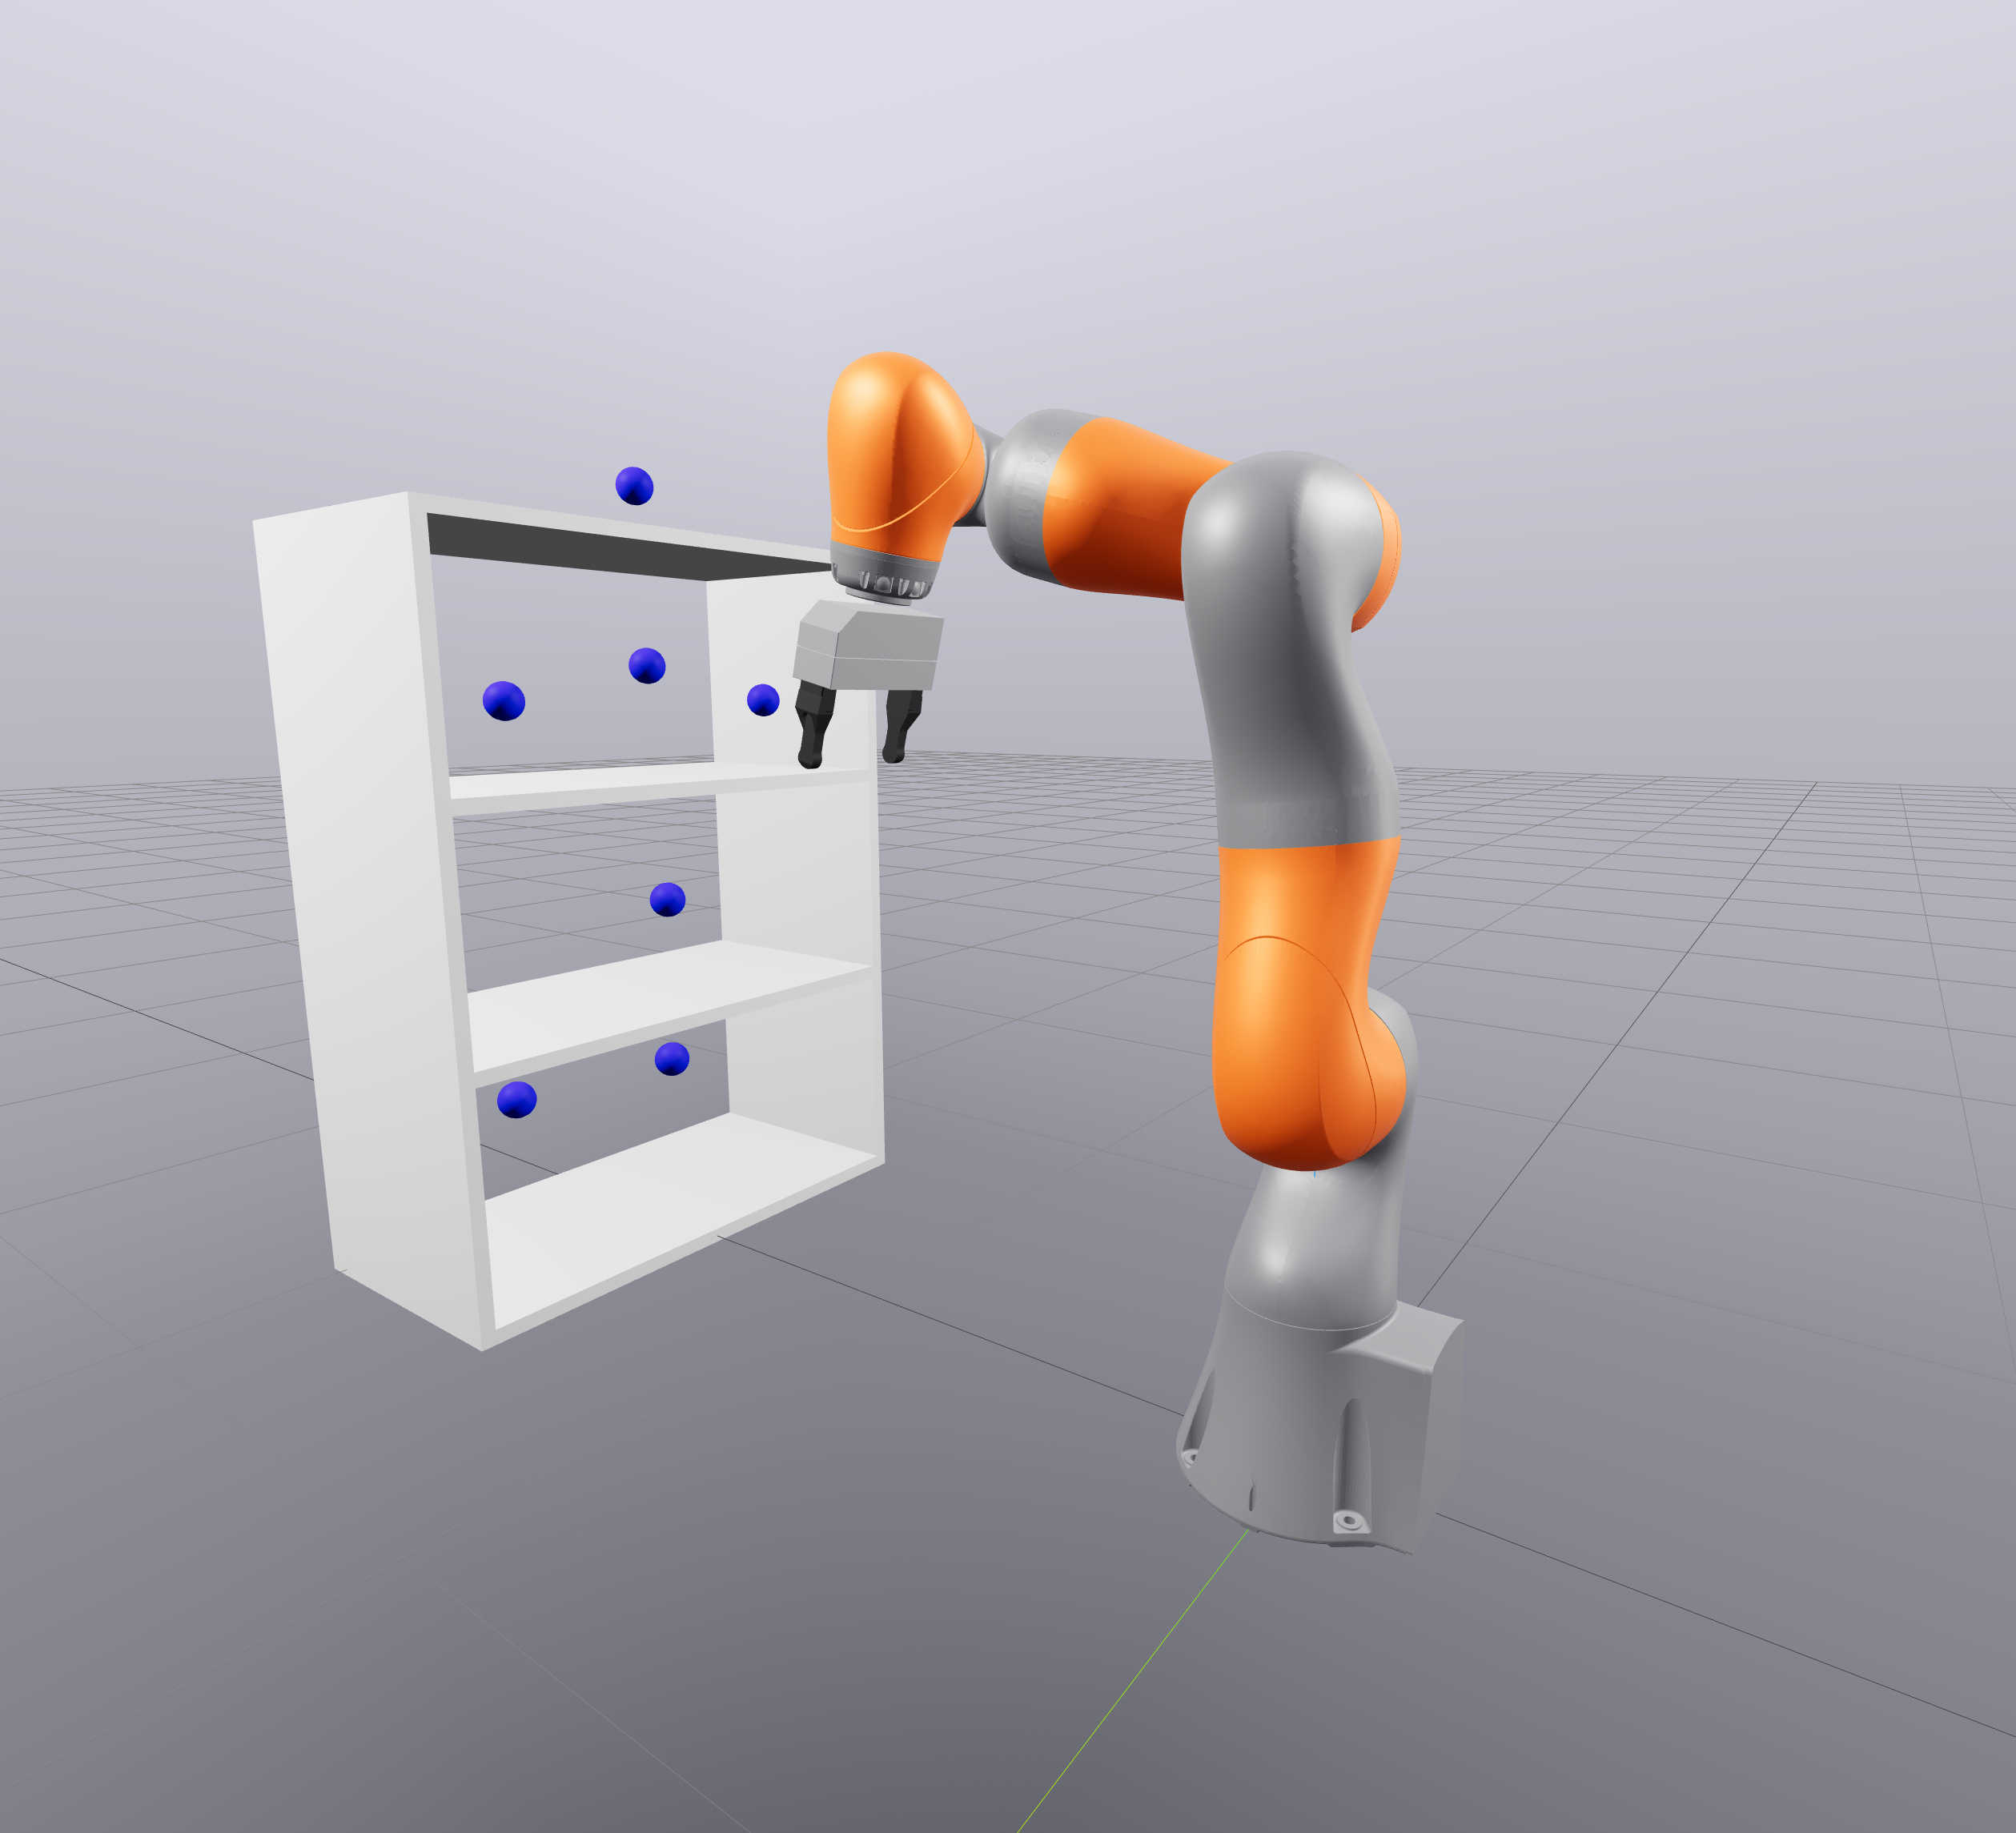
\includegraphics[
            height=3.5cm,
            keepaspectratio
        ]{pics/1sh.png}
        \caption{Одна полка}
    \end{subfigure}
    \hfill
    \begin{subfigure}[t]{0.32\textwidth}
        \centering
        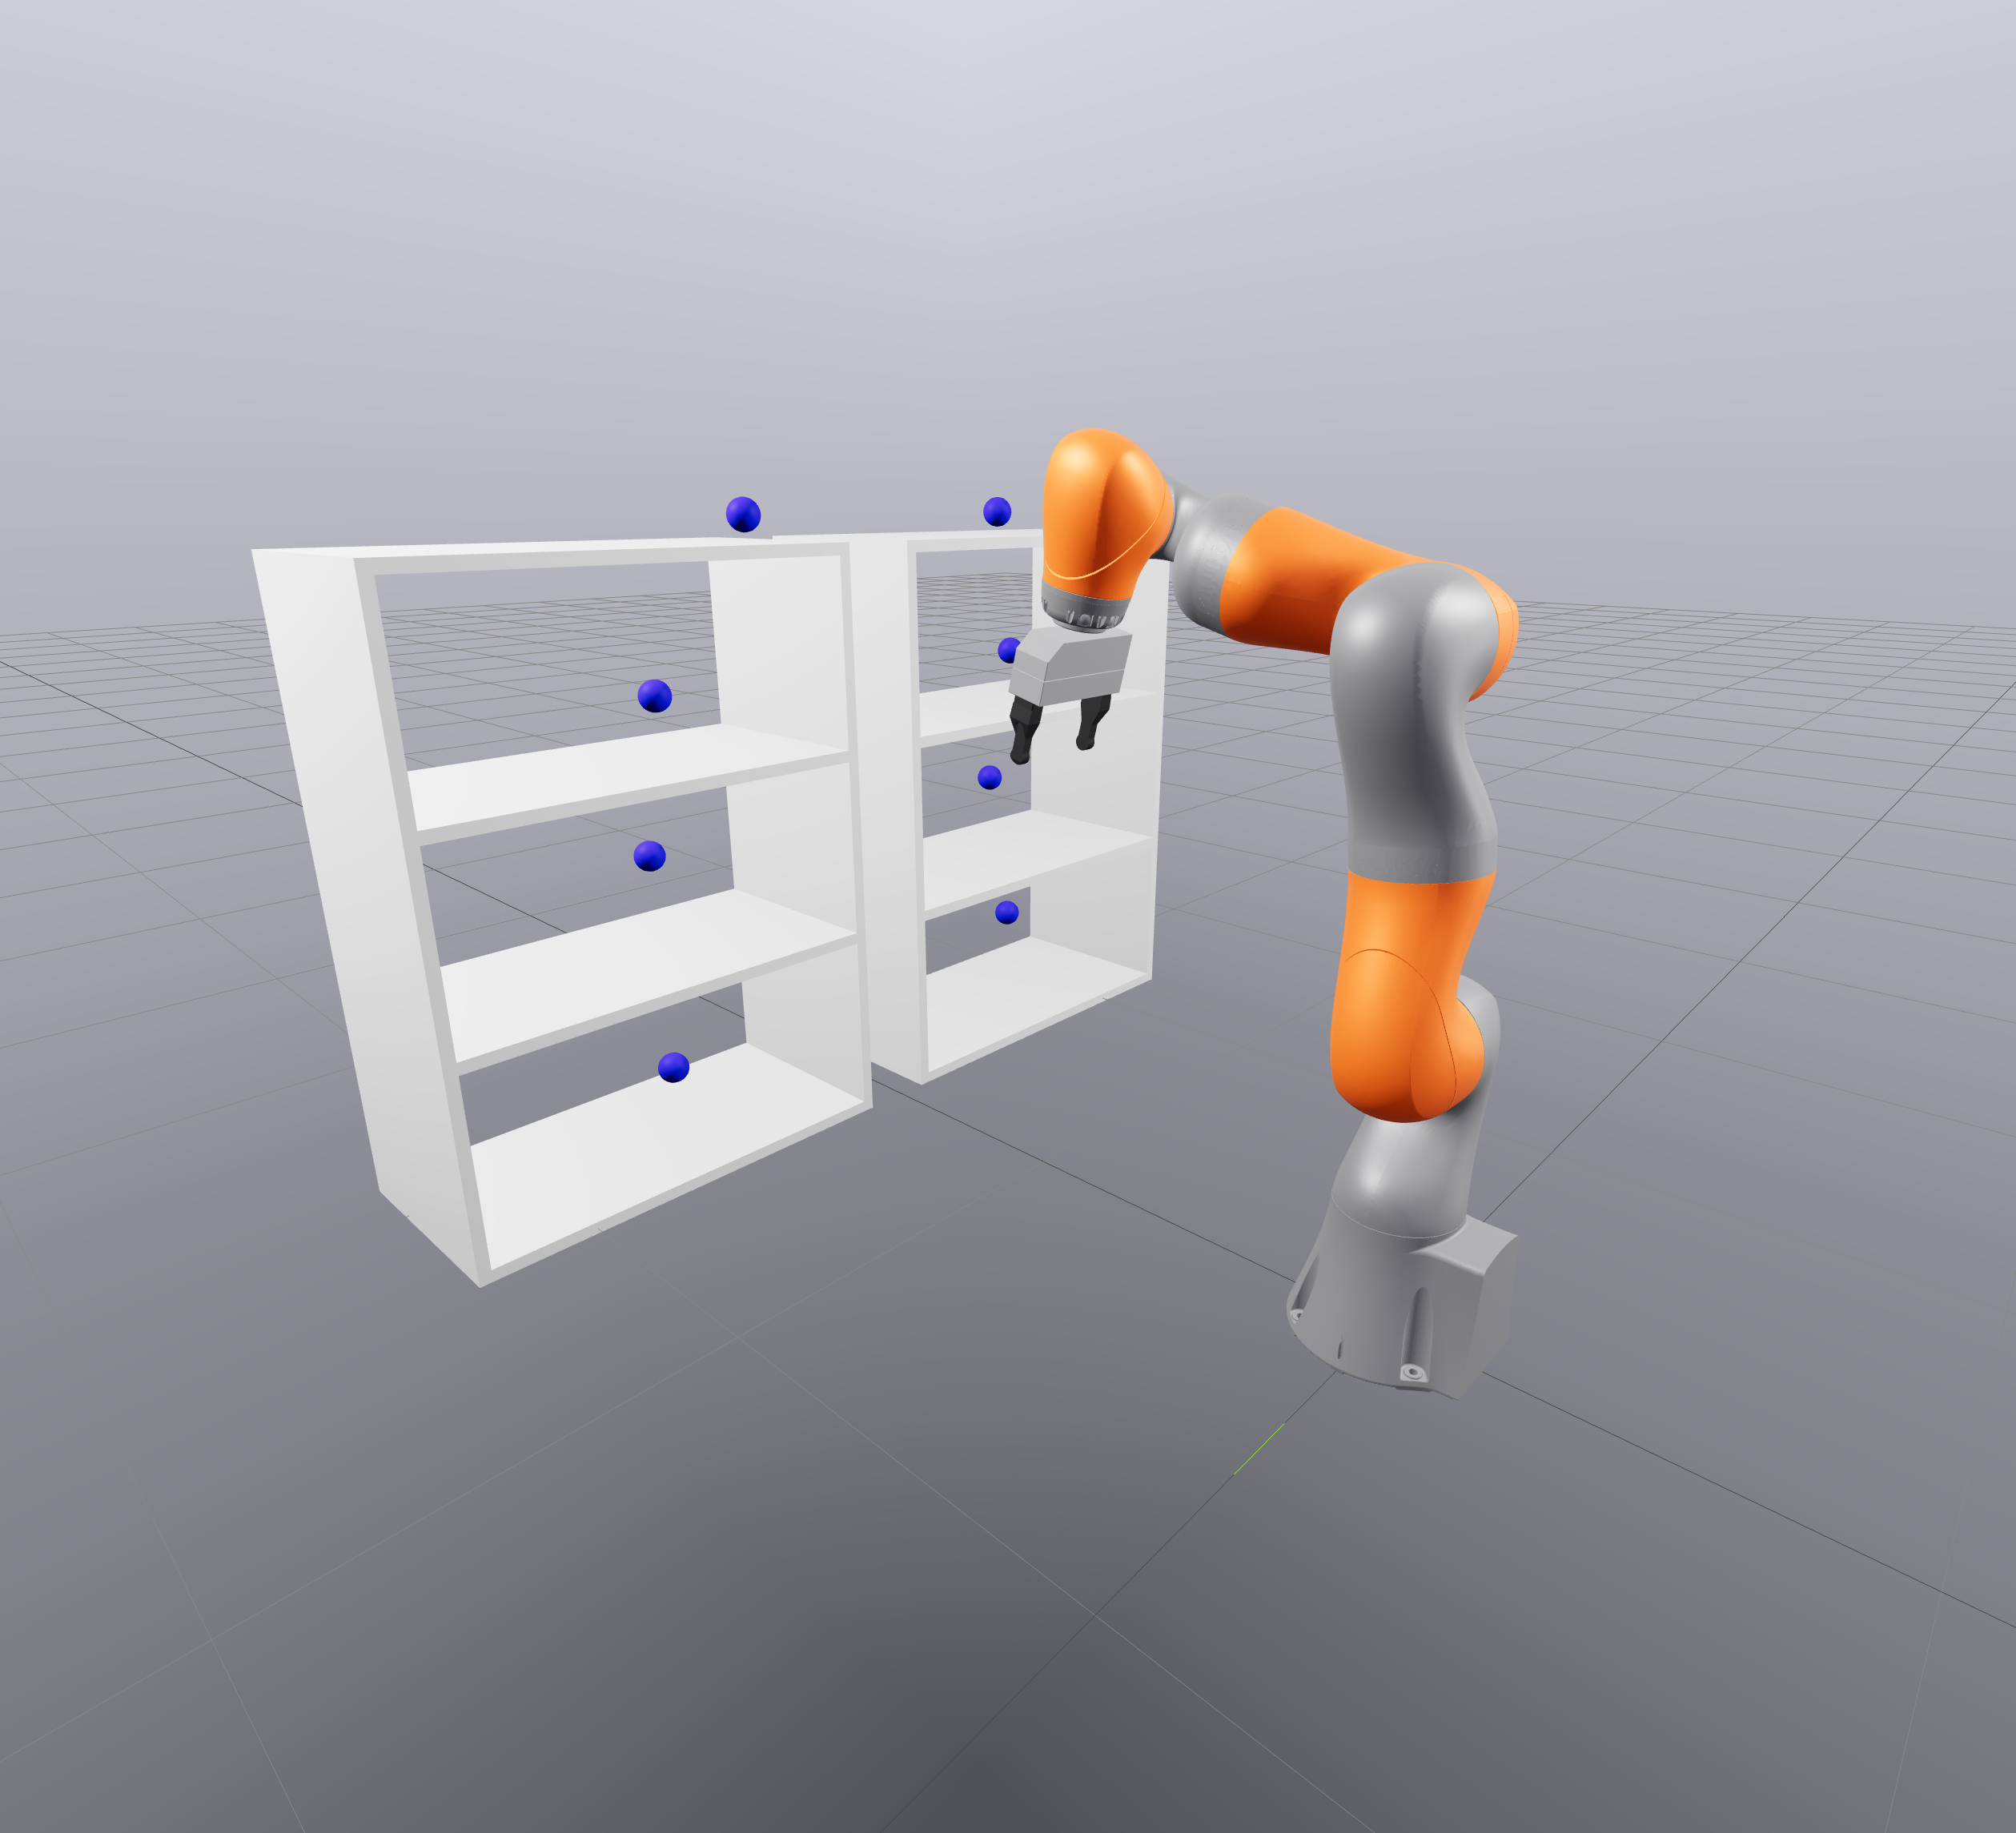
\includegraphics[
            height=3.5cm,
            keepaspectratio
        ]{pics/2sh.png}
        \caption{Две полки}
    \end{subfigure}
    \hfill
    \begin{subfigure}[t]{0.32\textwidth}
        \centering
        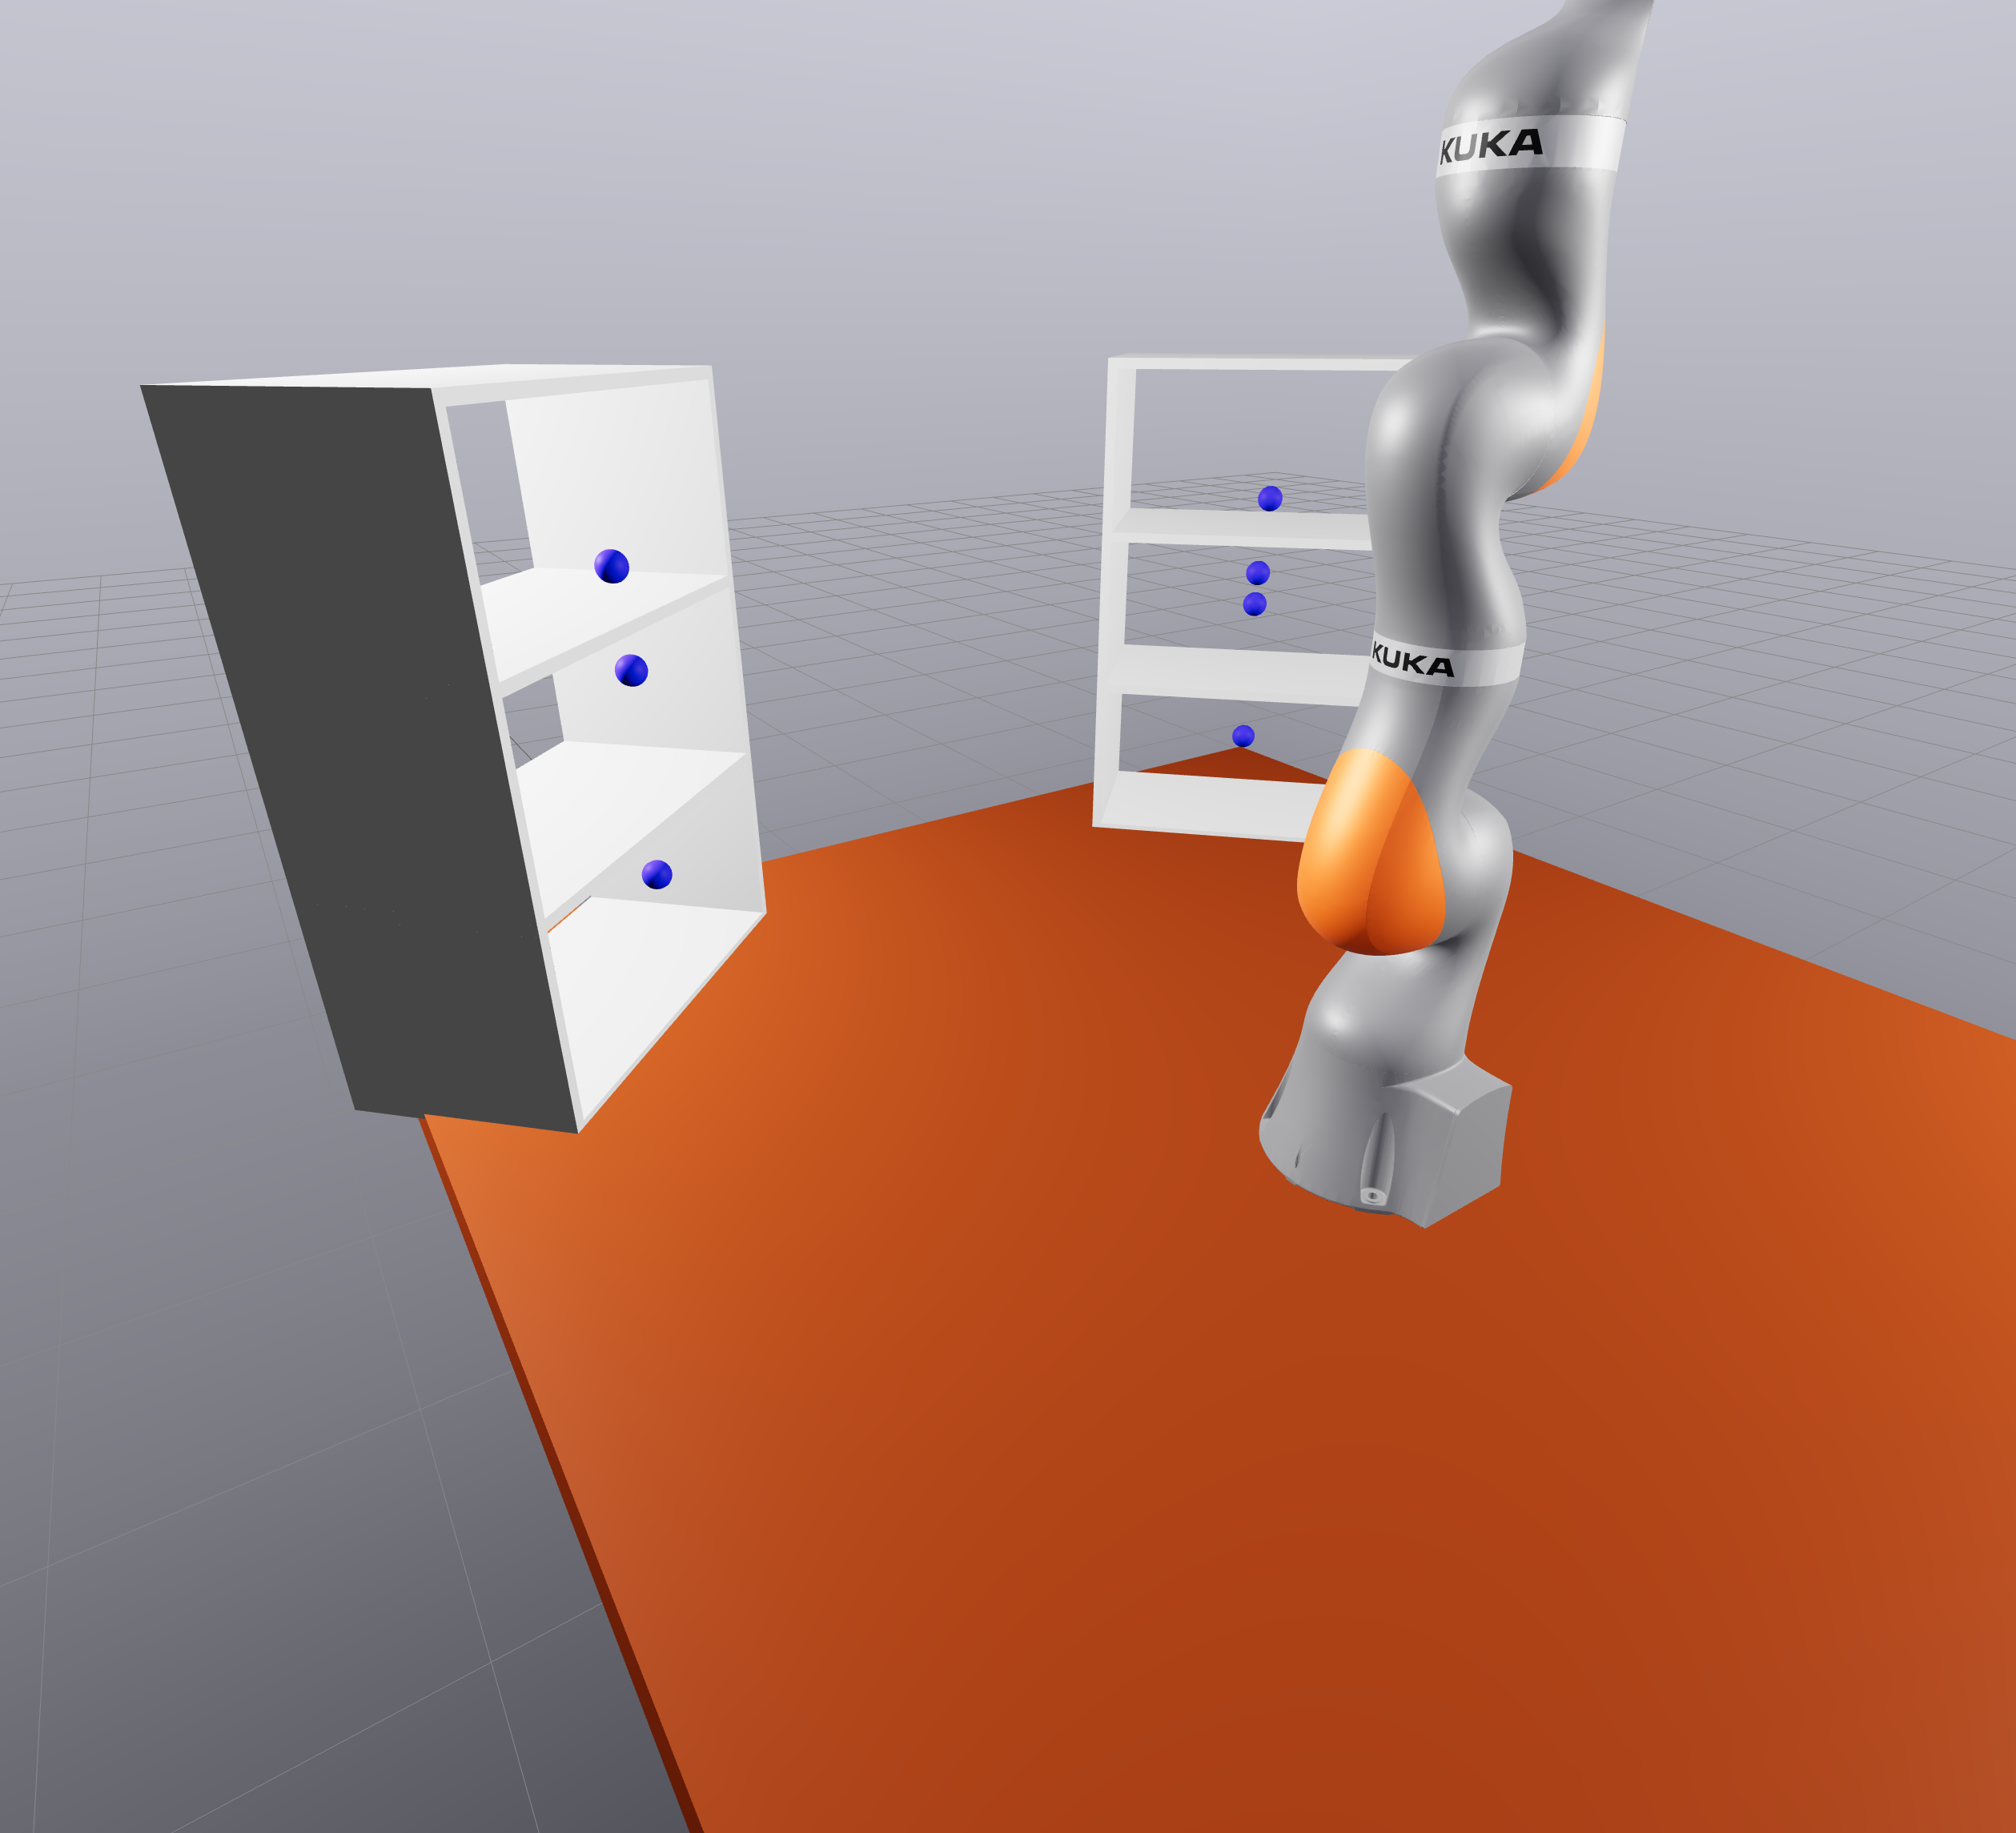
\includegraphics[
            height=3.5cm,
            keepaspectratio
        ]{pics/3sh.png}
        \caption{Три полки}
    \end{subfigure}

    \caption{Примеры начальных точек для построения IRIS-регионов в сценах с полками}
    \label{fig:shelf_start_points}
\end{figure}


\section{Результаты экспериментов}

\begin{table}[H]
\centering
\caption{GCS planning statistics by scene and number of seeds (regions). Failure breakdown is shown as counts of IRIS-region construction failures vs disconnected-region failures (No path). Abbreviations: SS --- Single Shelf, TS --- Two Shelves, 3S --- Three Shelves.}
\label{tab:success_results}
\begin{tabular}{l
                S[table-format=2.0]
                l
                S[table-format=2.0]
                S[table-format=2.0]
                l
                S[table-format=1.3]}
\toprule
\textbf{Scene} & \textbf{Seeds} & \textbf{Success} & \textbf{IRIS fail} & \textbf{No path} & \textbf{Path Length} & \textbf{Solve Time (s)} \\
\midrule
SS & 10 & 4/21  & 0  & 17 & 0.28 $\pm$ 0.08 & 0.003 \\
SS & 20 & 4/21  & 0  & 17 & 0.28 $\pm$ 0.08 & 0.003 \\
SS & 30 & 4/21  & 0  & 17 & 0.28 $\pm$ 0.08 & 0.003 \\
SS & 50 & 11/21 & 0  & 10 & 2.08 $\pm$ 2.20 & 0.019 \\
\addlinespace
TS & 10 & 0/28 & 13 & 15 & -- & \multicolumn{1}{c}{--} \\
TS & 20 & 0/28 & 13 & 15 & -- & \multicolumn{1}{c}{--} \\
TS & 30 & 0/28 & 13 & 15 & -- & \multicolumn{1}{c}{--} \\
TS & 50 & 0/28 & 13 & 15 & -- & \multicolumn{1}{c}{--} \\
\addlinespace
3S & 10 & 0/55 & 19 & 36 & -- & \multicolumn{1}{c}{--} \\
3S & 20 & 1/55 & 19 & 35 & 6.99 $\pm$ 0.00 & 0.100 \\
3S & 30 & 0/55 & 19 & 36 & -- & \multicolumn{1}{c}{--} \\
3S & 50 & 3/55 & 19 & 33 & 7.04 $\pm$ 1.55 & 0.080 \\
\bottomrule
\end{tabular}
\end{table}

\begin{table}[H]
\centering
\caption{Summary of RRT* $\rightarrow$ GCS experiments (pairs where both methods succeeded). Abbreviations: SS --- Single Shelf, TS --- Two Shelves, 3S --- Three Shelves.}
\label{tab:rrt_gcs_results_summary}
\begin{tabular}{l
                S[table-format=2.0]
                l
                l
                l
                l
                l}
\toprule
\textbf{Scene} & \textbf{Pairs} & \textbf{RRT* OK} & \textbf{GCS OK} & \textbf{RRT* length} & \textbf{GCS length} & \textbf{Improvement} \\
\midrule
SS & 21 & 21/21 & 16/21 & 10.53$\pm$8.14 & 4.52$\pm$3.43 & 40.8\%$\pm$30.2\% \\
TS & 28 & 28/28 & 16/28 & 9.24$\pm$3.26  & 5.48$\pm$2.84 & 40.7\%$\pm$28.1\% \\
3S & 32 & 32/32 & 14/32 & 10.85$\pm$4.66 & 5.38$\pm$1.69 & 45.9\%$\pm$16.1\% \\
\midrule
\textbf{TOTAL} & 81 & 81/81 & 46/81 & 10.18$\pm$5.69 & 5.11$\pm$2.76 & 42.3\%$\pm$25.5\% \\
\bottomrule
\end{tabular}
\end{table}

\begin{table}[H]
\centering
\caption{Runtime breakdown (mean, seconds)}
\label{tab:rrt_gcs_times_summary}
\begin{tabular}{l
                S[table-format=1.2]
                S[table-format=3.1]
                S[table-format=1.3]
                S[table-format=3.1]}
\toprule
\textbf{Scene} & \textbf{RRT* time} & \textbf{IRIS time} & \textbf{GCS time} & \textbf{Total} \\
\midrule
SS & 3.50 & 68.0  & 0.109 & 71.6 \\
TS & 0.14 & 156.3 & 0.153 & 156.6 \\
3S & 2.63 & 214.3 & 0.201 & 217.2 \\
\bottomrule
\end{tabular}
\end{table}

\end{document}